\documentclass[conference]{IEEEtran}
\IEEEoverridecommandlockouts

\usepackage{cite}
\usepackage{amsmath,amssymb,amsfonts}
\usepackage{graphicx}
\usepackage{textcomp}
\usepackage{xcolor}
\usepackage{colortbl}
\usepackage{booktabs}
\usepackage{tikz}
\usepackage{pgfplots}
\pgfplotsset{compat=1.18}
\usetikzlibrary{arrows.meta,positioning,shapes.geometric,fit}
\definecolor{ctitle}{HTML}{2c2739}
\definecolor{mypurple}{HTML}{d2cce1}
\def\BibTeX{{\rm B\kern-.05em{\sc i\kern-.025em b}\kern-.08em
    T\kern-.1667em\lower.7ex\hbox{E}\kern-.125emX}}

\begin{document}

\title{LVForge: PE Malware Detection from Strong Baselines to Deep Metric Learning\\
{\color{ctitle}A Continuity-Driven and Reproducible Study}}

\author{\IEEEauthorblockN{Ly Ngoc Vu}
\IEEEauthorblockA{\textit{Industrial University of Ho Chi Minh City} \\
Ho Chi Minh City, Vietnam \\
dezzhuge@gmail.com}}

\maketitle

\begin{abstract}
Windows PE malware detection is operationally sensitive because even small false-positive increases can create substantial analyst cost. Building on prior baseline-oriented work, this study examines whether objective design on a fixed Transformer backbone improves low-FPR behavior under class imbalance. We implement a unified Flax/JAX LVModel pipeline and compare five variants: baseline, ArcFace, Contrastive, Triplet, and Multi-Similarity. To emulate deployment pressure, training uses a 1:19 benign:malware regime (907:17,235), and evaluation reports aggregate metrics, operating-point metrics (TPR@FPR at $10^{-2}$, $10^{-3}$, $10^{-4}$), and imbalance-focused indicators (specificity, FPR, FNR, balanced accuracy, MCC). Across five seeds, Multi-Similarity shows the strongest overall profile (F1 $=0.9970\pm0.0028$, TPR@FPR$=10^{-2}$ $=0.9879\pm0.0078$, specificity $=0.9658\pm0.0353$, MCC $=0.9466\pm0.0457$), while ArcFace degrades at strict low-FPR points. The baseline remains competitive and stable. These findings indicate that objective selection can materially change deployment-relevant behavior even when the encoder backbone is unchanged.
\end{abstract}

\begin{IEEEkeywords}
malware detection, Windows PE, Transformer, deep metric learning, class imbalance, low-FPR evaluation
\end{IEEEkeywords}

\section{\textcolor{ctitle}{Introduction}}
Windows PE malware detection is an operationally constrained classification problem: high aggregate accuracy is not sufficient when false positives directly increase analyst workload. In practical SOC pipelines, model selection must be based on low-FPR behavior, not only global ranking metrics.

Our prior ATC 2024 study \cite{atc2024} already established strong baseline performance using classical machine learning and text-based deep learning. The remaining gap is objective-level behavior under strict operating points. This paper addresses the following research question:
\begin{quote}
\textit{On a shared Transformer backbone, which training objective provides the best trade-off between aggregate quality and low-FPR behavior under imbalance?}
\end{quote}

This manuscript is written as a continuity paper for first-time readers. It connects old and new stages in one coherent narrative and explicitly separates inherited components from new contributions.

\textbf{Contributions.}
\begin{enumerate}
\item A reproducible unified pipeline for baseline and DML variants, with one backbone and controlled objective changes.
\item Implementation-level documentation of LVModel and its Flax Transformer building blocks.
\item A low-FPR, imbalance-aware evaluation protocol with multi-seed statistical reporting.
\item Evidence-based deployment guidance on baseline versus DML objectives.
\end{enumerate}

The remainder of this paper is organized as follows: Section II maps prior and current scope, Section III details dataset/task settings, Section IV presents methodology, Section V defines the experimental protocol, Section VI reports results, and Sections VII--IX discuss implications, limitations, and conclusions.

\section{\textcolor{ctitle}{Project Continuity and Scope}}
Table~\ref{tab:scope_map} maps prior and current scopes to make the extension explicit.

\begin{table}[htbp]
\caption{Scope map between prior and current stages}
\centering
\scriptsize
\setlength{\tabcolsep}{3pt}
\resizebox{\columnwidth}{!}{%
\begin{tabular}{p{2.45cm}p{2.25cm}p{2.6cm}}
\toprule
\rowcolor{mypurple!55}
Component & Prior stage (ATC 2024) & Current stage (LVForge) \\
\midrule
Dataset & Multi-source PE collection and preprocessing & Reused and audited; source-level vs local-run accounting \\
Models & LR, RF, SVC, XGBoost, LSTM, BiLSTM, DistilBERT & Shared Flax/JAX Transformer baseline (LVModel) \\
Metric learning & Not included & ArcFace, Contrastive, Triplet, Multi-Similarity \\
Evaluation & Aggregate classification metrics & Multi-seed + threshold-aware low-FPR + imbalance metrics \\
Reproducibility & Experimental scripts/paper outputs & Unified \texttt{run\_all.py}, JSON aggregation, checkpoint artifacts \\
\bottomrule
\end{tabular}%
}
\label{tab:scope_map}
\end{table}

Accordingly, the novelty of this stage is an objective-controlled extension, rather than a replacement of the prior baseline study.

\section{\textcolor{ctitle}{Dataset and Task Setting}}
\subsection{Task Definition}
The task is binary malware detection from text-like PE representations, with label mapping \texttt{0}=\textit{benign}, \texttt{1}=\textit{malware}.

\subsection{Data Origin and Local Run Statistics}
Following \cite{atc2024}, samples originate from VX Underground, VirusShare, Softonic, and SourceForge. The local experimental file is \texttt{finData.csv} (\texttt{Texts}, \texttt{label}).

\begin{table}[htbp]
\caption{Dataset summary from source-level to current run}
\centering
\footnotesize
\begin{tabular}{lccc}
\toprule
\rowcolor{mypurple!55}
Data view & Benign & Malware & Ratio (B:M) \\
\midrule
Source-level (prior stage) & 17,150 & 17,235 & 1:1.00 \\
Current local \texttt{finData.csv} & 17,135 & 17,235 & 1:1.01 \\
Subsampled pool for training/eval & 907 & 17,235 & 1:19.00 \\
\bottomrule
\end{tabular}
\label{tab:dataset_summary}
\end{table}

Imbalance is intentionally induced by benign subsampling with benign proportion $r=0.05$:
\begin{equation}
N_{\text{benign,target}} = \left\lfloor \frac{r}{1-r} N_{\text{malware}} \right\rfloor.
\end{equation}
With $N_{\text{malware}}=17{,}235$, we obtain $N_{\text{benign,target}}=907$ and total $N=18{,}142$.

For each seed, data is shuffled then split 80/20; evaluation keeps full batches only (\texttt{batch\_size}=128), yielding 3,584 validation samples per seed.

To make feature semantics explicit, Table~\ref{tab:dataset_structure} lists representative PE-derived attributes. Table~\ref{tab:dataset_compare} provides context against widely cited malware datasets.

\begin{table*}[htbp]
\caption{DATASET STRUCTURE INFORMATION}
\centering
\scriptsize
\setlength{\tabcolsep}{4pt}
\begin{tabular}{p{2.8cm}p{7.6cm}p{1.8cm}p{3.7cm}}
\toprule
\rowcolor{mypurple!55}
Feature field & Description & Type & Example \\
\midrule
Filename & Executable file name & String & setup.exe \\
MD5 & File hash signature & String & d41d8cd98f00b204e9800998ecf8427e \\
File Size & Binary size in bytes & Number & 1048576 \\
Entropy & Byte-level entropy & Float & 6.72 \\
PE Header Machine & Machine architecture identifier & Number & 332 \\
PE Header Number of Sections & Sections count in PE header & Number & 3 \\
Sections & Parsed section-level metadata & Object & section name=.text; size=4096 \\
Import Table & Imported DLL/API symbols & Object & quazip.dll: extractFile, compressFile \\
Export Table & Exported symbols if available & Object / Null & NaN when absent \\
Type & Ground-truth label & String & Malware / Benign \\
\bottomrule
\end{tabular}
\label{tab:dataset_structure}
\end{table*}

\begin{table}[htbp]
\caption{COMPARING DATASET CHARACTERISTICS}
\centering
\footnotesize
\begin{tabular}{lccc}
\toprule
\rowcolor{mypurple!55}
Dataset & Benign & Malware & Total \\
\midrule
Android Malware Dataset & 9,476 & 5,560 & 15,036 \\
SOREL-20M \cite{sorel} & 8.6M & 11.4M & 20M \\
BODMAS \cite{bodmas} & 57,293 & 77,142 & 134,437 \\
Our dataset (source-level) & 17,150 & 17,235 & 34,385 \\
\bottomrule
\end{tabular}
\label{tab:dataset_compare}
\end{table}

Compared with very large corpora, this medium-scale setup is suitable for controlled objective-level ablations and frequent reproducible runs.

\section{\textcolor{ctitle}{Methodology}}
\subsection{Unified Pipeline}
All variants share preprocessing, tokenizer, backbone, optimizer schedule, split logic, and evaluation code. Only the objective/head branch changes. This design isolates the effect of the learning objective while limiting confounding implementation differences. Fig.~\ref{fig:pipeline} summarizes the pipeline.

\begin{figure*}[!t]
\centering
\resizebox{\textwidth}{!}{%
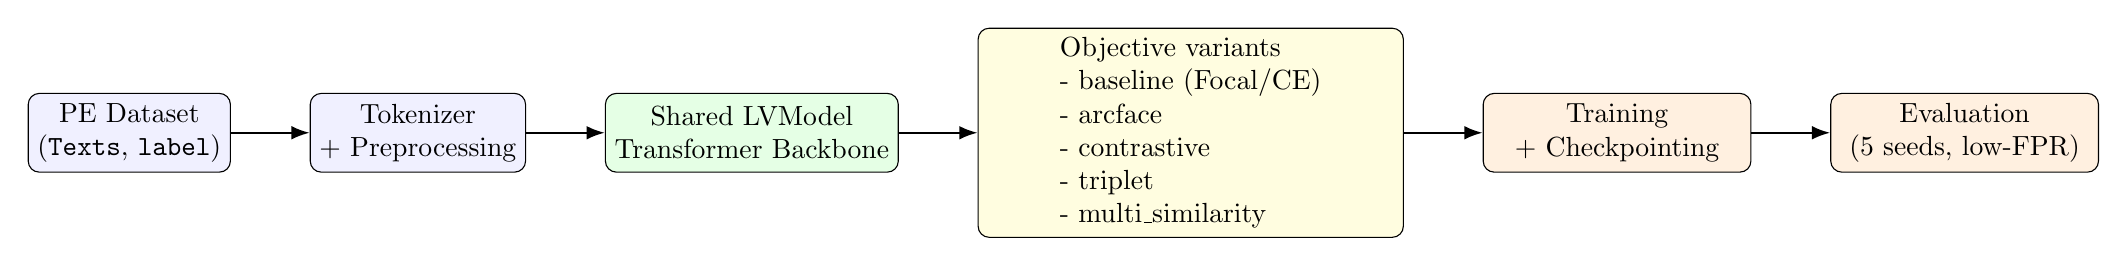
\begin{tikzpicture}[
    node distance=9mm and 10mm,
    stage/.style={draw, rounded corners, align=center, minimum height=10mm, minimum width=24mm, fill=blue!6},
    core/.style={draw, rounded corners, align=center, minimum height=10mm, minimum width=30mm, fill=green!10},
    block/.style={draw, rounded corners, align=left, minimum height=18mm, minimum width=54mm, fill=yellow!12},
    evalbox/.style={draw, rounded corners, align=center, minimum height=10mm, minimum width=34mm, fill=orange!12},
    arrow/.style={-Latex, thick}
]
    \node[stage] (data) {PE Dataset\\(\texttt{Texts}, \texttt{label})};
    \node[stage, right=of data] (prep) {Tokenizer\\+ Preprocessing};
    \node[core, right=of prep] (backbone) {Shared LVModel\\Transformer Backbone};
    \node[block, right=of backbone] (heads) {Objective variants\\- baseline (Focal/CE)\\- arcface\\- contrastive\\- triplet\\- multi\_similarity};
    \node[evalbox, right=of heads] (train) {Training\\+ Checkpointing};
    \node[evalbox, right=of train] (eval) {Evaluation\\(5 seeds, low-FPR)};

    \draw[arrow] (data) -- (prep);
    \draw[arrow] (prep) -- (backbone);
    \draw[arrow] (backbone) -- (heads);
    \draw[arrow] (heads) -- (train);
    \draw[arrow] (train) -- (eval);
\end{tikzpicture}}
\caption{Unified pipeline for baseline and DML variants.}
\label{fig:pipeline}
\end{figure*}

\subsection{LVModel Architecture Details}
The shared encoder is implemented with \texttt{FlaxMultiHeadSelfAttention} and \texttt{FlaxTransformerLayer} modules. For input IDs $\mathbf{X}\in\mathbb{N}^{B\times T}$:
\begin{equation}
\mathbf{H}_0 = E_{\text{tok}}(\mathbf{X}) + E_{\text{pos}}(1{:}T).
\end{equation}

Each Transformer block uses pre-normalization residual connections:
\begin{align}
\tilde{\mathbf{H}} &= \mathrm{LN}(\mathbf{H}_{l-1}), \\
\mathbf{H}' &= \mathbf{H}_{l-1} + \mathrm{MHA}(\tilde{\mathbf{H}}), \\
\mathbf{H}_{l} &= \mathbf{H}' + \mathrm{FFN}(\mathrm{LN}(\mathbf{H}')).
\end{align}

In attention, Q/K/V are generated by a single dense projection:
\begin{equation}
\mathrm{QKV}=W_{qkv}\mathbf{H}, \quad
\mathbf{A}=\mathrm{softmax}\left(\frac{QK^\top}{\sqrt{d_h}}\right).
\end{equation}

Sequence representations are mean-pooled, then passed through dense+tanh, dropout, LayerNorm, and a linear classifier:
\begin{equation}
\mathbf{z}=\frac{1}{T}\sum_{t=1}^{T}\mathbf{H}_{L,t}.
\end{equation}

Configuration: $d_{\text{model}}=256$, heads$=8$, $d_{ff}=512$, layers$=2$, dropout$=0.1$, max length$\approx380$.

\subsection{Objective Heads and Losses}
\textbf{Baseline.} The baseline uses the same LVModel with focal loss \cite{focal} during training:
\begin{equation}
\mathcal{L}_{\text{focal}}=-\alpha(1-p_t)^\gamma\log(p_t),
\end{equation}
with $\alpha=0.25$, $\gamma=2.0$.

\textbf{ArcFace.} ArcFace \cite{arcface} applies additive angular margin in cosine space:
\begin{equation}
\mathcal{L}_{\text{arc}}=-\log\frac{e^{s\cos(\theta_y+m)}}{e^{s\cos(\theta_y+m)}+\sum_{j\neq y}e^{s\cos(\theta_j)}}.
\end{equation}

\textbf{Contrastive/Triplet/Multi-Similarity.} These variants use normalized embeddings and optimize a hybrid objective:
\begin{equation}
\mathcal{L}=\lambda\mathcal{L}_{\text{CE}}+(1-\lambda)\mathcal{L}_{\text{metric}},
\end{equation}
with $\lambda=0.5$ in this implementation for Contrastive, Triplet (batch-hard), and Multi-Similarity \cite{contrastive,triplet,msloss}.

\section{\textcolor{ctitle}{Experimental Protocol}}
\subsection{Reproducible Setup}
All variants are launched by one command:
\begin{quote}
\texttt{python scripts/run\_all.py}
\end{quote}
The latest full run finished with 5/5 PASS in 558.6 seconds.

Common setup:
\begin{itemize}
\item Seeds: \{42, 43, 44, 45, 46\}.
\item Batch size: 128; epochs: 5; early stopping patience: 2.
\item Optimizer: AdamW with cosine decay and gradient clipping.
\item Learning rate: $2\times10^{-4}$.
\item Split: shuffled 80/20 validation protocol per seed.
\end{itemize}

\subsection{Metrics and Thresholding}
Thresholds are tuned per seed by maximizing validation F1 on the PR curve. Reported metrics include Accuracy, Precision, Recall, F1, ROC-AUC, PR-AUC, TPR@FPR($10^{-2}$, $10^{-3}$, $10^{-4}$), and imbalance-focused metrics:
\begin{align}
\text{Specificity} &= \frac{TN}{TN+FP}, \\
\text{FPR} &= \frac{FP}{FP+TN}, \\
\text{FNR} &= \frac{FN}{FN+TP}, \\
\text{MCC} &= \frac{TP\cdot TN-FP\cdot FN}{\sqrt{(TP+FP)(TP+FN)(TN+FP)(TN+FN)}}.
\end{align}
For each metric, we report mean and sample standard deviation over five seeds, and compute 95\% confidence intervals using a $t$-interval. This reporting choice is intended to emphasize operational stability rather than single-run point performance.

\section{\textcolor{ctitle}{Results}}
\subsection{Prior-Stage Reference}
Tables~\ref{tab:prior_ml} and \ref{tab:prior_dl} provide prior-stage results from \cite{atc2024}. They are included for context and continuity, not direct protocol-matched comparison.

\begin{table}[htbp]
\caption{ML baselines from prior paper \cite{atc2024}}
\centering
\footnotesize
\begin{tabular}{lcccc}
\toprule
\rowcolor{mypurple!55}
Model & Precision & Recall & F1 & Accuracy \\
\midrule
Logistic Regression & 0.990086 & 0.990232 & 0.990111 & 0.990112 \\
Random Forest & 0.990000 & 0.990382 & 0.990402 & 0.990403 \\
SVC & 0.990000 & 0.988060 & 0.988075 & 0.988076 \\
XGBoost & 0.990000 & 0.991542 & 0.991566 & 0.991566 \\
\bottomrule
\end{tabular}
\label{tab:prior_ml}
\end{table}

\begin{table}[htbp]
\caption{Deep learning baselines from prior paper \cite{atc2024}}
\centering
\footnotesize
\begin{tabular}{lcccc}
\toprule
\rowcolor{mypurple!55}
Model & Precision & Recall & F1 & Accuracy \\
\midrule
DistilBERT & 0.9864895 & 0.9865220 & 0.9864705 & 0.986471 \\
LSTM & 0.9674135 & 0.9674490 & 0.9674130 & 0.967413 \\
BiLSTM & 0.9507005 & 0.9499545 & 0.9500705 & 0.950102 \\
\bottomrule
\end{tabular}
\label{tab:prior_dl}
\end{table}

\subsection{Current LVForge Results (5-Seed Mean $\pm$ Std)}
\begin{table}[htbp]
\caption{Objective-level comparison on the current pipeline}
\centering
\scriptsize
\setlength{\tabcolsep}{3pt}
\resizebox{\columnwidth}{!}{%
\begin{tabular}{lccccccc}
\toprule
\rowcolor{mypurple!55}
Variant & Acc & F1 & ROC-AUC & PR-AUC & TPR@1e-2 & TPR@1e-3 & TPR@1e-4 \\
\midrule
baseline & 0.9923$\pm$0.0040 & 0.9959$\pm$0.0021 & 0.9983$\pm$0.0016 & 0.9999$\pm$0.0001 & 0.9754$\pm$0.0157 & 0.9468$\pm$0.0512 & 0.9468$\pm$0.0512 \\
arcface & 0.9858$\pm$0.0018 & 0.9925$\pm$0.0009 & 0.9643$\pm$0.0053 & 0.9981$\pm$0.0002 & 0.0000$\pm$0.0000 & 0.0000$\pm$0.0000 & 0.0000$\pm$0.0000 \\
contrastive & 0.9942$\pm$0.0050 & 0.9969$\pm$0.0026 & 0.9971$\pm$0.0040 & 0.9998$\pm$0.0004 & 0.9830$\pm$0.0132 & 0.7151$\pm$0.3431 & 0.7151$\pm$0.3431 \\
triplet & 0.9928$\pm$0.0060 & 0.9962$\pm$0.0032 & 0.9979$\pm$0.0029 & 0.9999$\pm$0.0002 & 0.9768$\pm$0.0176 & 0.9146$\pm$0.0883 & 0.9146$\pm$0.0883 \\
multi\_similarity & \textbf{0.9944$\pm$0.0053} & \textbf{0.9970$\pm$0.0028} & \textbf{0.9984$\pm$0.0022} & \textbf{0.9999$\pm$0.0001} & \textbf{0.9879$\pm$0.0078} & \textbf{0.9561$\pm$0.0316} & \textbf{0.9561$\pm$0.0316} \\
\bottomrule
\end{tabular}%
}
\label{tab:current_main}
\end{table}

\begin{table}[htbp]
\caption{Imbalance-focused metrics (5 seeds)}
\centering
\scriptsize
\resizebox{\columnwidth}{!}{%
\begin{tabular}{lccccc}
\toprule
\rowcolor{mypurple!55}
Variant & Specificity & FPR & FNR & Balanced Acc & MCC \\
\midrule
baseline & 0.9387$\pm$0.0372 & 0.0613$\pm$0.0372 & 0.0047$\pm$0.0020 & 0.9670$\pm$0.0195 & 0.9236$\pm$0.0348 \\
arcface & 0.8802$\pm$0.0813 & 0.1198$\pm$0.0813 & 0.0086$\pm$0.0026 & 0.9358$\pm$0.0395 & 0.8567$\pm$0.0310 \\
contrastive & 0.9533$\pm$0.0434 & 0.0467$\pm$0.0434 & \textbf{0.0035$\pm$0.0027} & 0.9749$\pm$0.0230 & 0.9430$\pm$0.0449 \\
triplet & 0.9439$\pm$0.0326 & 0.0561$\pm$0.0326 & 0.0045$\pm$0.0045 & 0.9697$\pm$0.0183 & 0.9303$\pm$0.0504 \\
multi\_similarity & \textbf{0.9658$\pm$0.0353} & \textbf{0.0342$\pm$0.0353} & 0.0040$\pm$0.0036 & \textbf{0.9809$\pm$0.0193} & \textbf{0.9466$\pm$0.0457} \\
\bottomrule
\end{tabular}%
}
\label{tab:imbalance}
\end{table}

\begin{table}[htbp]
\caption{Runtime from latest full run (\texttt{run\_all.py})}
\centering
\footnotesize
\begin{tabular}{lc}
\toprule
\rowcolor{mypurple!55}
Variant & Time (s) \\
\midrule
baseline & 93.6 \\
arcface & 100.0 \\
contrastive & 122.5 \\
triplet & 125.8 \\
multi\_similarity & 116.7 \\
\bottomrule
\end{tabular}
\label{tab:runtime}
\end{table}

\begin{table}[htbp]
\caption{Welch $t$-test: Multi-Similarity vs baseline (n=5)}
\centering
\footnotesize
\begin{tabular}{lcc}
\toprule
\rowcolor{mypurple!55}
Metric & Mean diff. (MS - Base) & $p$-value \\
\midrule
F1 & +0.0011 & 0.5014 \\
TPR@FPR=1e-2 & +0.0124 & 0.1659 \\
TPR@FPR=1e-3 & +0.0093 & 0.7402 \\
Specificity & +0.0271 & 0.2715 \\
MCC & +0.0230 & 0.3997 \\
\bottomrule
\end{tabular}
\label{tab:ttest}
\end{table}

Overall, the results indicate that objective choice affects low-FPR behavior more strongly than aggregate metrics alone suggest. Multi-Similarity maintains favorable operating-point behavior, whereas ArcFace appears sensitive under strict false-positive constraints.

\section{\textcolor{ctitle}{Discussion}}
\textbf{RQ1: Does deep metric learning help on imbalanced PE data?} Yes, but not uniformly across objectives. Multi-Similarity is strongest overall in this run, while ArcFace underperforms at strict low-FPR points despite acceptable aggregate scores.

\textbf{RQ2: Is baseline still useful?} Yes. The baseline remains strong and stable, and can be treated as a robust deployment fallback.

\textbf{RQ3: Why not claim strict superiority yet?} The sample size is limited (five seeds), and Table~\ref{tab:ttest} reports non-significant differences between baseline and Multi-Similarity. This aligns with overlapping confidence intervals and indicates that the practical advantage is promising but not definitive.

\textbf{Operational implication.} Objective choice strongly affects low-FPR behavior. Deployment screening should therefore include TPR@FPR, specificity, FNR, and MCC in addition to Accuracy/F1/AUC.

\section{\textcolor{ctitle}{Threats to Validity and Limitations}}
\textbf{Internal validity.} Validation uses shuffled 80/20 splits with fixed seed set, not an external hold-out.

\textbf{External validity.} Results are from one medium-scale PE corpus; transferability to other malware families, time periods, and packing/obfuscation regimes is untested.

\textbf{Statistical conclusion validity.} Although five-seed reporting improves robustness over single-run comparisons, statistical power remains limited for small effect sizes.

\section{\textcolor{ctitle}{Conclusion}}
This continuity paper consolidates inherited baseline foundations and new objective-level extensions in LVForge. Under controlled comparison on a shared backbone, Multi-Similarity provides the strongest operating profile in this run, while baseline remains a stable reference model. Future work should validate these trends on external or temporal hold-out data and include calibration analysis before stronger deployment claims are made.

\section*{Acknowledgment}
This work extends the author's previous study and reframes the pipeline for reproducible objective-level analysis for new supervision context.

\begin{thebibliography}{00}
\bibitem{atc2024} L. N. Vu, ``Windows Malware Detection: Exploring from Machine Learning to Text-Based Deep Learning Approaches,'' in Proc. ATC, 2024.
\bibitem{focal} T.-Y. Lin \textit{et al.}, ``Focal Loss for Dense Object Detection,'' ICCV, 2017.
\bibitem{arcface} J. Deng \textit{et al.}, ``ArcFace: Additive Angular Margin Loss for Deep Face Recognition,'' CVPR, 2019.
\bibitem{msloss} X. Wang \textit{et al.}, ``Multi-Similarity Loss with General Pair Weighting for Deep Metric Learning,'' CVPR, 2019.
\bibitem{triplet} F. Schroff \textit{et al.}, ``FaceNet: A Unified Embedding for Face Recognition and Clustering,'' CVPR, 2015.
\bibitem{contrastive} R. Hadsell \textit{et al.}, ``Dimensionality Reduction by Learning an Invariant Mapping,'' CVPR, 2006.
\bibitem{sorel} A. Harang and E. M. Rudd, ``SOREL-20M: A Large Scale Benchmark Dataset for Malicious PE Detection,'' arXiv:2012.07634, 2020.
\bibitem{bodmas} BODMAS Dataset, ``Benchmark for malware analysis at scale,'' 2021.
\end{thebibliography}

\end{document}
